% LTeX: language=en-US

\documentclass[handout,usepdftitle=false,xcolor=dvipsnames,aspectratio=169]{beamer}
%\documentclass[beamer,usepdftitle=false,xcolor=dvipsnames,aspectratio=169]{beamer}
%\documentclass[trans,notes=show,usepdftitle=false,aspectratio=169]{beamer}


\usepackage[english]{babel}
\usepackage{iftex}
\ifPDFTeX
\usepackage[T1]{fontenc}
\usepackage[utf8]{inputenc}
\usepackage{lmodern}
\else
\usepackage{fontspec}
\defaultfontfeatures{Ligatures=TeX}
\setmainfont{Latin Modern Roman}
\setsansfont{Latin Modern Sans}
\setmonofont{Latin Modern Mono}
\usepackage{newunicodechar}
\newfontfamily\unicodeSymbolFont{Segoe UI Symbol}[
  BoldFont=Segoe UI Symbol,
  ItalicFont=Segoe UI Symbol,
  BoldItalicFont=Segoe UI Symbol
]
\newunicodechar{⟂}{{\unicodeSymbolFont ⟂}}
\fi
\usepackage{amsmath,amsfonts}
\usepackage{booktabs,multirow,xcolor,colortbl}
\usepackage{bm}%to use a more powerful version of \boldsymbol
\usepackage{fvextra}
\usepackage{csquotes}
\usepackage{textcomp}
\ifPDFTeX
\DeclareUnicodeCharacter{27C2}{\ensuremath{\perp}}
\fi

\newcommand{\AllSample}{ \mathcal Y^T }

\usepackage[citestyle=authoryear-comp,bibstyle=../Preamble/mystyle_lowercase,maxbibnames=5,minbibnames=1,maxnames=2, minnames=1,datezeros=false,date=long,isbn=false,url=false,backend=biber,useprefix=true]{biblatex}
\addglobalbib{../Preamble/Macro_database_biblatex.bib}	

\usepackage{upquote}
\usepackage{ragged2e}
\usepackage{microtype}

\usepackage{multimedia}
\usepackage{graphicx}
\usepackage[export]{adjustbox}
\usepackage{epstopdf}
\usepackage[labelfont=bf,format=hang, figurename=Fig.]{caption}
\usepackage[subrefformat=parens,labelformat=empty]{subcaption}
\usepackage{pgfpages} % for multiple-screen presentations

\usepackage{array}

\newcolumntype{L}[1]{>{\RaggedRight\let\newline\\\arraybackslash\hspace{0pt}}m{#1}}
\newcolumntype{C}[1]{>{\centering\let\newline\\\arraybackslash\hspace{0pt}}m{#1}}
\newcolumntype{R}[1]{>{\raggedleft\let\newline\\\arraybackslash\hspace{0pt}}m{#1}}
%https://tex.stackexchange.com/questions/12703/how-to-create-fixed-width-table-columns-with-text-raggedright-centered-raggedlef


%%% use serif font for math
\usefonttheme[onlymath]{serif}

%%% define blue highlighting
\newcommand{\highlight}[1]{{\color{blue}{#1}}}

%%%% define command for setting sources

\newcommand{\Source}{}

%%%
\beamertemplatenavigationsymbolsempty


%%% define themes
\usetheme{Boadilla}
\usecolortheme{rose}
\usecolortheme[named=blue]{structure}

\newcommand\textbox[1]{%
  \parbox{.333\textwidth}{#1}%
}

\setbeamertemplate{sections/subsections in toc}[sections numbered]


%%%% set coloring in  foot and head
\setbeamercolor{alerted text}{fg=red!80!black}
\setbeamertemplate{enumerate items}[default] % numbers enumerate items without encircling them
\setbeamertemplate{itemize items}[ball] % numbers enumerate items without encircling them
\setbeamercolor{section in head/foot}{fg=black, bg=white}
\setbeamercolor{subsection in head/foot}{fg=black, bg=white}
\setbeamercolor{title}{fg=black}
\setbeamercolor{subtitle}{fg=blue}

\setbeamertemplate{caption}[numbered]

%%% set overlays as default
\beamerdefaultoverlayspecification{<+->}

%%%% settings for output mode

\mode<beamer>
{
%\setbeameroption{show notes on second screen=right}
}

\mode<trans>
{\renewcommand{\highlight}[1]{{\textbf{#1}}}}


\mode<handout>
{
\renewcommand{\highlight}[1]{{\textbf{#1}}}
%\pgfpagesuselayout{4 on 1}[a4paper,border shrink = 5mm,landscape]
%\setbeamercolor{background canvas}{bg=black!5}
}


%%% define Exercise counter
\newcounter{Exercise}
\resetcounteronoverlays{Exercise}
\setcounter{Exercise}{0}
\newcommand{\Exercise}{\refstepcounter{Exercise}\emph{\structure{Übung \theExercise}: }}

%%%% define environments for theorems etc and make them numbered
\setbeamertemplate{theorems}[numbered]

\newtheorem{assum}{Assumption}
\setbeamertemplate{assum}[numbered]

\newtheorem{defin}{Definition}
\setbeamertemplate{defin}[numbered]

\newtheorem{propos}{Proposition}
\setbeamertemplate{propos}[numbered]


%%%% Make Parts show up in TOC
\makeatletter
\AtBeginPart{%
  \addtocontents{toc}{\protect\beamer@partintoc{\the\c@part}{\beamer@partnameshort}{\the\c@page}}%
}
%% number, shortname, page.
\providecommand\beamer@partintoc[3]{%
  \ifnum\c@tocdepth=-1\relax
    % requesting onlyparts.
    \makebox[6em]{#1.} #2
    \par
  \fi
}
\define@key{beamertoc}{onlyparts}[]{%
  \c@tocdepth=-1\relax
}
\makeatother%

%%%% fix bug in beamer package with note itemize
%%% http://tex.stackexchange.com/questions/1480/changing-the-textwidth-of-the-notes-in-beamer-repost-from-so
\makeatletter
\defbeamertemplate{note page}{infolines}
{%
  \vskip.75em
  \nointerlineskip
  \begin{minipage}{\textwidth} % this is an addition
  \footnotesize \insertnote
  \end{minipage}               % this is an addition
}
\makeatother

\setbeamertemplate{note page}[infolines]


\newcommand{\backupbegin}{
   \newcounter{framenumberappendix}
   \setcounter{framenumberappendix}{\value{framenumber}}
}
\newcommand{\backupend}{
   \addtocounter{framenumberappendix}{-\value{framenumber}}
   \addtocounter{framenumber}{\value{framenumberappendix}}
}

\hypersetup{bookmarksnumbered=true,naturalnames=true,pdfhighlight=/N,citebordercolor={1 1
1},linkbordercolor={1 1 1},colorlinks=true,anchorcolor=black,linkcolor=blue,citecolor=green,urlcolor=green,
pdfpagemode=UseOutlines,breaklinks=true,
pdfkeywords=Dynare, pdfsubject=Dynare,pdfstartpage=1} %pdfpagemode=fullpage

\usepackage[copyright]{ccicons}

\usepackage{tikz,pgfplots}
\pgfplotsset{compat=1.18}
\usetikzlibrary{arrows,calc,decorations.pathreplacing,decorations.shapes}
\pgfdeclarelayer{background}
\pgfdeclarelayer{foreground}
\pgfsetlayers{background,main,foreground}

\usepackage{relsize}
\newcommand\LM{\ensuremath{\mathit{LM}}}
\newcommand\IS{\ensuremath{\mathit{IS}}}
\DeclareMathOperator{\std}{std}


\setbeamertemplate{footline}{
\begin{beamercolorbox}{subsection in head/foot}
\insertsectionnavigationhorizontal{.95\textwidth}{\hskip0pt
\hfill}{\hfill \insertframenumber /\inserttotalframenumber}
\end{beamercolorbox}
}

\newenvironment{witemize}{\itemize\addtolength{\itemsep}{8pt}}{\enditemize}
\newenvironment{wenumerate}{\enumerate\addtolength{\itemsep}{8pt}}{\endenumerate}

\usepackage[]{minted}
\usepackage{tcolorbox}
\usepackage{etoolbox}
\BeforeBeginEnvironment{minted}{\begin{tcolorbox}[boxsep=0mm]}%
\AfterEndEnvironment{minted}{\end{tcolorbox}}%

\AtBeginEnvironment{minted}{%
  \renewcommand{\fcolorbox}[4][]{#4}}  

\begin{document}

%\inserttotalframenumber


\title[]{\textbf{Advanced Dynare\\}
  \medskip{Chapter X}\\
  \emph{Forecasting}
}

\author{Johannes Pfeifer}
\input{../date_place.txt}

\AtBeginSection[]
{
  \begin{frame}
    \frametitle{Outline}
    \tableofcontents[currentsection]
  \end{frame}
}


\maketitle
%\include{Intro}
\begin{frame}
  \frametitle{Outline}
  \tableofcontents%[onlyparts]
\end{frame}



\section{Introduction}

\begin{frame}{Motivation}
  \begin{witemize}
    \item Structural models are often used for forecasting exercises
    \item \textcite{SmetsWouters2007}: performance on par with time series techniques
    \item Dynare provides a variety of tools to perform such exercises
    \item Important conceptual distinctions:
    \begin{enumerate}
      \item conditional vs. unconditional forecasting
      \item stochastic vs. perfect foresight forecasting
      \item point forecast vs. density forecast
    \end{enumerate}
  \end{witemize}
\end{frame}



\section[Stochastics w/o parameter uncertainty]{Stochastic models without parameter uncertainty}


\begin{frame}{Forecasting based on recursive policy rules}
  \begin{witemize}
    \item Perturbation solutions with \texttt{stoch\_simul} yield recursive policy rules for the endogenous variables $x_{t-1}$ of the form
    \begin{equation}
      y_t = g(x_{t-1},\varepsilon_t|\theta) \: ,
    \end{equation}
    where
    \begin{itemize}
      \item $x_{t-1}$ are endogenous state variables
      \item $\varepsilon_t$ are exogenous state variables
      \item $\theta$ are structural models parameters
    \end{itemize}
    \item Given initial conditions $x_{T}$ and sequence of future shocks $\varepsilon_{T+i},i=\{1,\ldots,h\}$, we can compute future path of all endogenous variables $y_t$\\
    $\rightarrow$ conditional forecasts require selecting specific $\varepsilon_{T+i}$ 
    \item Drawing from distribution of shocks for $\varepsilon_{T+i}$ allows generating density forecasts that take shock uncertainty into account\\
    $\rightarrow$ no parameter uncertainty as calibration $\theta$ is given
  \end{witemize}
\end{frame}

\subsection{Unconditional forecasts}

\begin{frame}[fragile]{Basic unconditional forecast: Dynare code I}{\texttt{rbc\_basic\_forecast.mod}}
  \begin{itemize}
    \item Consider again the basic RBC model with AR(1) technology shocks:
  \end{itemize}
  \begin{minted}{c++}
model;
  c + k = exp(A)*k(-1)^alpha + (1-delta)*k(-1);
  c^(-gamma) = 
    beta*c(+1)^(-gamma)*(alpha*exp(A(+1))*k^(alpha-1) + 1-delta);
  A= rho*A(-1)+epsilon;
end;

steady_state_model;
  A = 0;
  k = ((1-beta*(1-delta))/(beta*alpha*exp(A)))^(1/(alpha-1));
  c = exp(A)*k^alpha-delta*k;
end;
steady;
\end{minted}
\end{frame}


\begin{frame}[fragile]{Basic unconditional forecast: Dynare code II}{\texttt{rbc\_basic\_forecast.mod}}
  \begin{itemize}
    \item \texttt{forecast} command currently only allow first order approximatiom\\
    $\rightarrow$ should change for Dynare 7
    \item Define the shock distribution and solve the model at first order:
  \end{itemize}
  \begin{minted}{c++}
shocks;
  var epsilon=0.01^2;
end;

stoch_simul(order=1,irf=0);
\end{minted}
\end{frame}

\begin{frame}[fragile]{Basic unconditional forecast: Dynare code III}{\texttt{rbc\_basic\_forecast.mod}}
  \begin{itemize}
    \item We can set the initial condition for the state variable $k$ to be 5\% below its steady state value using \texttt{histval}-block
    \item The \texttt{forecast} command allows computing a 100-period density forecast with 95\% confidence intervals
  \end{itemize}
  \begin{minted}{c++}
ik = varlist_indices('k',M_.endo_names);
kstar = oo_.steady_state(ik);

histval;
  k(0) = kstar*0.95;
end;

forecast(periods=100,conf_sig=0.95);
\end{minted}
\end{frame}

\begin{frame}[fragile]{Basic unconditional forecast: Dynare output}{\texttt{rbc\_basic\_forecast.mod}}
  \begin{figure}
    \centering
    
\includegraphics[width=0.7\textwidth]{examples/rbc_basic_forecast/graphs/forcst1.eps}
  \end{figure}
  \begin{itemize}
    \item Results are stored in the \texttt{oo\_.forecast} field
  \end{itemize}
\end{frame}

\begin{frame}[fragile]{Deterministic exogenous shocks}{\texttt{rbc\_basic\_forecast\_varexo\_det.mod}}
  \begin{witemize}
    \item Perturbation solutions up to \texttt{order=2} allow having deterministic exogenous shocks in addition to stochastic shocks (implementation details at \href{https://git.dynare.org/Dynare/dynare/-/wikis/varexo_det:-Implementation}{Dynare Wiki})\\
    $\rightarrow$ deterministic exogenous shocks become known with certainty at time $T$
    \item \texttt{varexo\_det} statement declares deterministic exogenous shocks
    \begin{minted}{c++}
varexo_det eps_det;
...
model;
...
A= rho*A(-1)+epsilon + eps_det;
end;
\end{minted}
  \end{witemize}
\end{frame}

\begin{frame}[fragile]{Deterministic exogenous shocks: Dynare code}{\texttt{rbc\_basic\_forecast\_varexo\_det.mod}}
  \begin{itemize}
    \item perfect foresight-type syntax allows specifying the realization period and value of the deterministic shocks
  \end{itemize}
  \begin{minted}{c++}
shocks;
  var epsilon=0.01^2;
  var eps_det; periods 8; values 1;
end;

stoch_simul(order=1,irf=0);

forecast(periods=20,conf_sig=0.95);
\end{minted}
\end{frame}

\begin{frame}[fragile]{Deterministic exogenous shocks: Dynare output}{\texttt{rbc\_basic\_forecast\_varexo\_det.mod}}
  \begin{figure}
    \centering
    
\includegraphics[width=0.7\textwidth]{examples/rbc_basic_forecast_varexo_det/graphs/forcst1.eps}
  \end{figure}
  \begin{itemize}
    \item Deterministic shock occurs in period 8 and is known with certainty at the time of forecasting
    \item Works like a news shock \parencite[e.g.][]{BeaudryPortier2006}\\
          $\rightarrow$ forward-looking agents react to it already before it materializes
  \end{itemize}
\end{frame}

\subsection{Conditional forecasts}


\begin{frame}{Conditional forecasts}
  \begin{witemize}
    \item Policy-makers are often interested in conditional forecasts, i.e.\ forecasts given future paths of some endogenous variable(s)
    \item Example: what happens if we set nominal interest rate to zero for the next 2 quarters?
    \item Achieving given future path of endogenous variables requires solving for shocks that generate this path\\
    $\rightarrow$ requires as many shocks as controlled endogenous variables
    \item Having more shocks and computing most likely linear combination can be achieved with Kalman filter-type algorithm \parencite[e.g.][]{BanburaEtAl2015}, but is not (yet) implemented in Dynare
  \end{witemize}
\end{frame}

\begin{frame}{Conditional forecasts: setup}
  \begin{witemize}
    \item Relies on state-space form from first-order perturbation solution:
    \begin{equation}
      y_t = T y_{t-1} + R \varepsilon_t
    \end{equation}
    \item Without loss of generality, at time $t$ both $y_t$ and $\varepsilon_t$ can be split into controlled (top) and uncontrolled (bottom):
    \begin{equation}
      \begin{pmatrix} y_{1,t} \\ y_{2,t} \end{pmatrix} =
      \begin{pmatrix} T_{11} & T_{12} \\ T_{21} & T_{22} \end{pmatrix}
      \begin{pmatrix} y_{1,t-1} \\ y_{2,t-1} \end{pmatrix} +
      \begin{pmatrix} R_{11} & R_{12} \\ R_{21} & R_{22} \end{pmatrix}
      \begin{pmatrix} \varepsilon_{1,t} \\ \varepsilon_{2,t} \end{pmatrix} \ ,
    \end{equation}
    where $y_{1,t}$ are ``controlled'' endogenous variables and $\varepsilon_{1,t}$ are controlled shocks
    \item Goal: solve linear system for $\varepsilon_{1,t}$ to get desired $y_{1,t}$\\
    $\rightarrow$ no unique solution to the problem for higher order approximation, e.g.\ quadratic equation
  \end{witemize}
\end{frame}

\begin{frame}{Conditional forecasts: Algorithm}
  \begin{witemize}
    \item At time $t$, we
    \begin{itemize}
      \item  know past states $y_{1,t}, y_{2,t}$ and random realization of uncontrolled shocks $\varepsilon_{2,t}$
      \item are given the desired values for controlled endogenous variables $y_{1,t}$
    \end{itemize}
    \item We can solve the first block of the matrix equation to obtain:
    \begin{equation}
      \varepsilon_{1,t} = R_{11}^{-1} \left( y_{1,t} - T_{11}y_{1,t-1} - T_{12}y_{2,t-1} - R_{12}\varepsilon_{2,t} \right)
    \end{equation}
    \item Shock inversion requires matrix $R_{11}$ to be square and full rank:
    \begin{itemize}
      \item number of controlled shocks equal to number of constrained endogenous variables
      \item controlled shocks must independently affect the controlled endogenous variables\\
            $\rightarrow$ no ``redundant'' shocks
    \end{itemize}
    \item Given $\varepsilon_{1,t}$, unconstrained endogenous variables $y_{2,t}$ can be updated by evaluating the second block of equations:
    \begin{equation}
      y_{2,t} = T_{21}y_{1,t-1} + T_{22}y_{2,t-1} + R_{21}\varepsilon_{1,t} + R_{22}\varepsilon_{2,t}
    \end{equation}
  \end{witemize}
\end{frame}

\begin{frame}[fragile]{Conditional forecasts: Dynare code I}{\texttt{NK\_linear\_controlled\_forecast.mod}}
  \begin{itemize}
    \item Consider linear New Keynesian model with 3 exogenous shocks:
  \end{itemize}
  \small
  \begin{minted}{c++}
model(linear);
[name='Phillips Curve']   
pie=betta*pie(+1)+kappa*y+eps_a;
[name='DIS curve']
y=y(+1)-1/sig*(inom-pie(+1))+eps_c;
[name='Nominal interest rate Taylor rule']
inom=phi_pi*pie+phi_y*y+eps_i;   
[name='Law of motion for cost-push shocks']
eps_a=rho_a*eps_a(-1)+u_a;
[name='Law of motion for demand shocks']
eps_c=rho_c*eps_c(-1)+u_c;
[name='Law of motion for interest-rate shocks']
eps_i=rho_i*eps_i(-1)+u_i;
end;
\end{minted}
\end{frame}

\begin{frame}[fragile]{Conditional forecasts: Dynare code II}{\texttt{NK\_linear\_controlled\_forecast.mod}}
  \begin{itemize}
    \item Set up stochastic shock distribution and compute decision rules at first order:
  \end{itemize}
  \small
  \begin{minted}{c++}
shocks;
    var u_c  = 0.005^2;   
    var u_a  = 0.005^2; 
    var u_i  = 0.005^2; 
end;
stoch_simul(order = 1,irf=0) y pie inom ;
\end{minted}
\end{frame}

\begin{frame}[fragile]{Conditional forecasts: Dynare code III}{\texttt{NK\_linear\_controlled\_forecast.mod}}
  \begin{itemize}
    \item Use \texttt{conditional\_forecast\_paths;} block to set nominal interest rate path over the next 5 periods 
    \item Request forecast using \texttt{conditional\_forecast} command, defining controlled shock set using the \texttt{controlled\_varexo} option
    \item Plot the results using \texttt{plot\_conditional\_forecast} command
  \end{itemize}
  \small
  \begin{minted}{c++}
conditional_forecast_paths;
var inom;
periods  1  2  3:5;
values   0.01 0.02 0.1;
end;

conditional_forecast(parameter_set=calibration, controlled_varexo=(u_i));
plot_conditional_forecast(periods=10) inom y;
\end{minted}
\end{frame}

\begin{frame}[fragile]{Conditional forecasts: Dynare output}{\texttt{NK\_linear\_controlled\_forecast.mod}}
  \begin{figure}
    \centering
    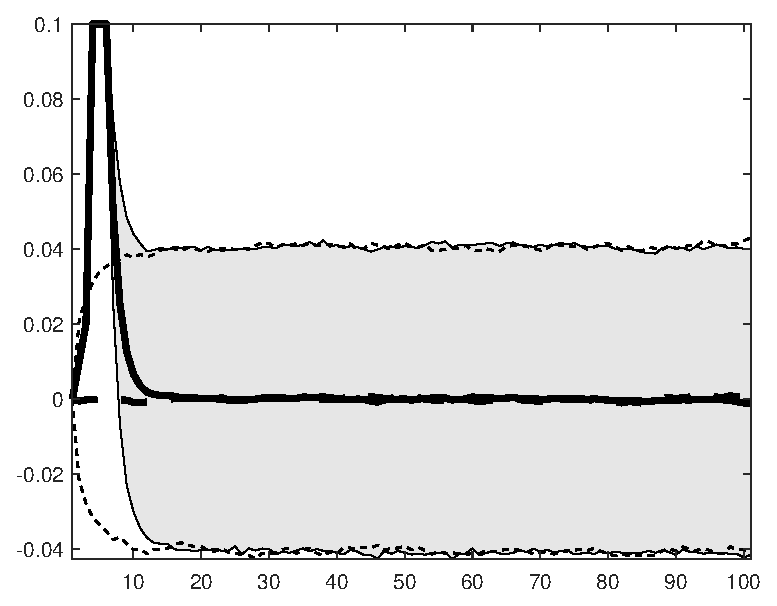
\includegraphics[width=0.4\textwidth]{examples/NK_linear_controlled_forecast/graphs/Conditional_forecast_Calibration_inom.eps}
    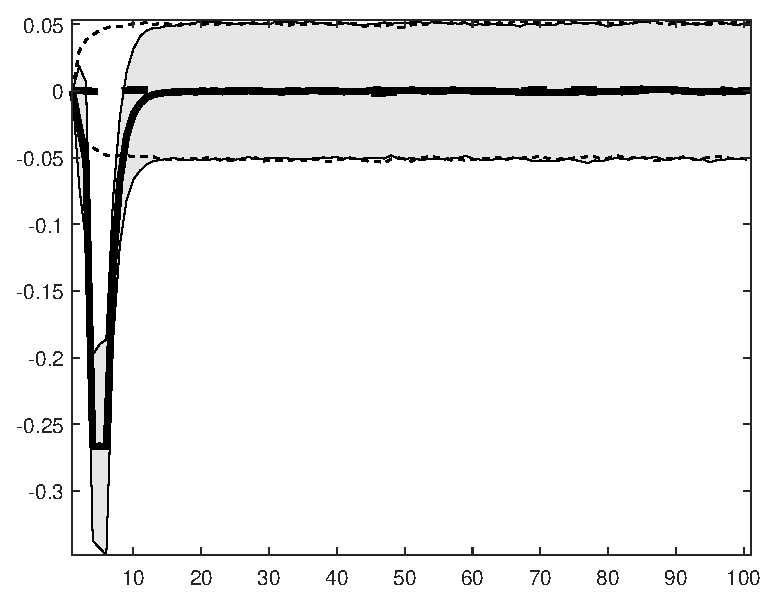
\includegraphics[width=0.4\textwidth]{examples/NK_linear_controlled_forecast/graphs/Conditional_forecast_Calibration_y.eps}
  \end{figure}
  \begin{itemize}
    \item Results are stored in the \texttt{oo\_.conditional\_forecast} field
    \item Plots show both conditional forecast (solid line) and unconditional forecast (dashed line) with \texttt{conf\_sig}\% confidence intervals
  \end{itemize}
\end{frame}

\subsection{Calibrated smoother}

\begin{frame}{Dealing with unobserved states}
  \begin{witemize}
    \item Forecasting scenarios usually involve conditioning on the state of the economy at the end of the available sample $T$
    \item Problem: while agents in RE models know the true state, econometrician does not
    \item Otherwise, we could simply put everything we need in the \texttt{histval} block as before
    \item Need to infer the relevant state variables $x_{T}$ at the end of the sample from some data\\
    $\rightarrow$ filtering/smoothing problem
    \item Most commonly, this is done in a linear/first-order perturbation framework where well-known techniques can be efficiently exploited
  \end{witemize}
\end{frame}

\begin{frame}{Linear models: Kalman filter/smoother}
  \begin{witemize}
    \item For a given parameter set $\theta$, the linear law of motion of states
    \begin{equation}
      x_{t + 1} = F x_t + w_{t + 1}
    \end{equation}
    implies:
    \begin{equation}
      x_{T+h|T} = F^h x_{T|T} + \sum_{j=1}^h F^{h-j} w_{T+j|T}
    \end{equation}
    \item In linear Gaussian world, the Kalman filter/smoother naturally constructed optimal estimates of the states given observed data\\
    $\rightarrow$ yields initial condition $x_{T|T}$
    \item We could also directly use the Kalman filter recursions at the end of the sample to obtain the filtered estimates $x_{T+h|T}$ for $h>0$

  \end{witemize}
\end{frame}

\begin{frame}[fragile]{Calibrated smoother: Dynare code}{\texttt{rbc\_basic\_calib\_smoother.mod}}
  \begin{itemize}
    \item Simulate artificial data and use it as the \texttt{datafile} to the \texttt{calib\_smoother} command
    \item Request $k$-step ahead filtered variables and plot them
  \end{itemize}
  \small
  \begin{minted}{c++}
stoch_simul(order=1,irf=0,periods=200) c;

datatomfile ('rbc_data', {'c'});
varobs c;

calib_smoother(datafile='rbc_data',filter_step_ahead=[1:8]);
for var_iter=1:8
    forecast_c(var_iter)=oo_.FilteredVariablesKStepAhead
      (var_iter,varlist_indices('c',M_.endo_names),200+var_iter);
end
figure
plot(1:8,forecast_c);
title('C, based on filter_step_ahead','Interpreter','none')
\end{minted}
\end{frame}

\begin{frame}[fragile]{Calibrated smoother forecasts: Code and output}{\texttt{rbc\_basic\_calib\_smoother.mod}}
  \begin{figure}
    \centering
    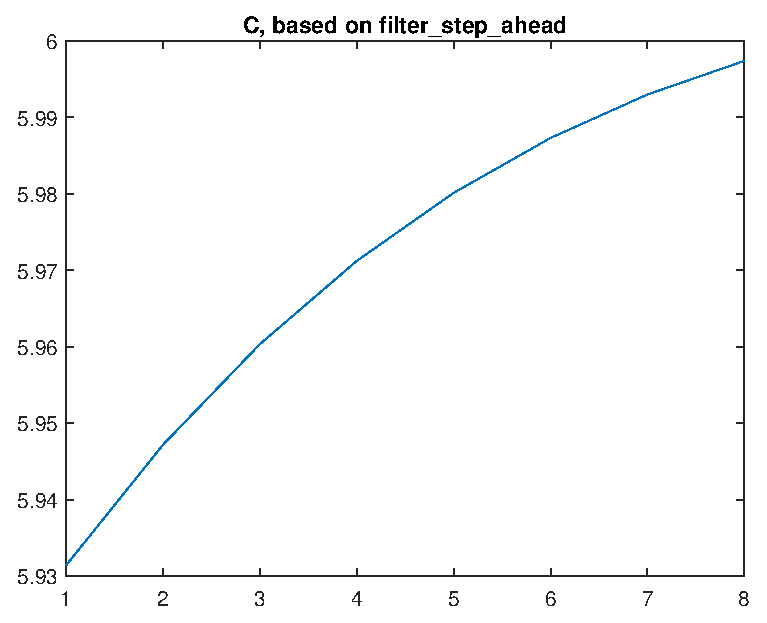
\includegraphics[width=0.3\textwidth]{examples/rbc_basic_calib_smoother/graphs/c_forecast.eps}
    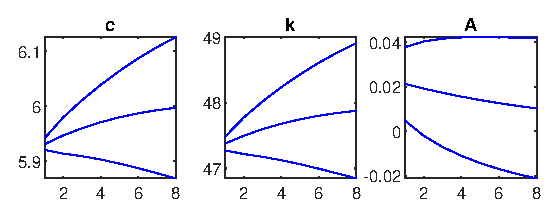
\includegraphics[width=0.6\textwidth]{examples/rbc_basic_calib_smoother/graphs/forcst1.eps}
  \end{figure}
  \begin{itemize}
    \item Better way: use \texttt{smoother2histval} function to set
          \texttt{histval} block based on the smoothed states at time $T$ from \texttt{calib\_smoother}
    \item Use \texttt{forecast} command as before to compute conditional forecast:
  \end{itemize}
  \small
  \begin{minted}{c++}
smoother2histval;
forecast(periods=8);
\end{minted}
\end{frame}

\section[Stochastics parameter uncertainty]{Stochastic models without parameter uncertainty}

\begin{frame}{Parameter uncertainty}
  \begin{witemize}
    \item In many applications, parameter uncertainty is an important source of uncertainty for forecasts\\
    $\rightarrow$ comes on top of disturbance uncertainty
    \item We saw how to estimate the parameters of a DSGE model\\
    $\rightarrow$ characterized posterior distribution using MCMC
    \item Also saw how Monte Carlo integration over posterior allows evaluating integrals:
    \begin{equation}
      \mathbb{E}\left( {g\left( \theta  \right)|{y^T}} \right) = \int {g\left( \theta  \right)p\left( {\theta |{y^T}} \right)d\theta }  \approx \frac{1}{S}\sum\limits_{s = 1}^S {g\left( {{\theta _s}} \right)} =\hat g_S
    \end{equation}
    \item As $g(\theta)$ can be any function of $\theta$, it naturally encompasses forecasts $x_{T+h|T}$
  \end{witemize}
\end{frame}

\begin{frame}[fragile]{Posterior forecasting: Dynare code}{\texttt{rbc\_basic\_posterior\_forecast.mod}}
  \begin{itemize}
    \item Estimate the model parameters at first order
    \item Request $8$-step ahead \texttt{forecast}
  \end{itemize}
  \small
  \begin{minted}{c++}
varobs c;

estimated_params;
rho, 0.9, beta_pdf,0.7,0.1;
end;

estimation(order=1,datafile=rbc_data,forecast=8,
            mh_nblocks=1,mh_replic=4000,consider_all_endogenous);
\end{minted}
\end{frame}

\begin{frame}[fragile]{Posterior forecasting: Dynare output}{\texttt{rbc\_basic\_posterior\_forecast.mod}}

  \begin{figure}
\centering

\begin{subfigure}{0.5\textwidth}
\centering
    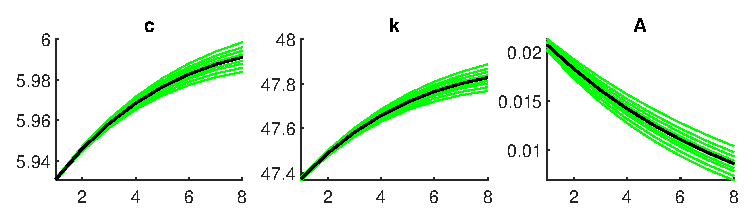
\includegraphics[width=\textwidth]{examples/rbc_basic_posterior_forecast/Output/rbc_basic_posterior_forecast_MeanForecast_A.eps}
\caption{Mean forecasts}
\end{subfigure}%
\begin{subfigure}{0.5\textwidth}
\centering
  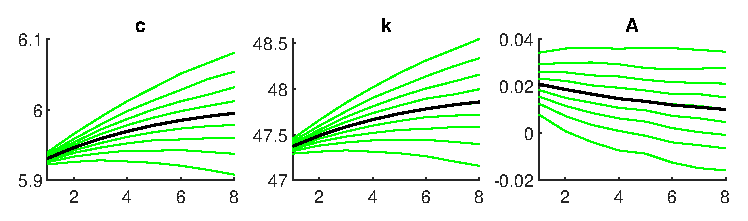
\includegraphics[width=\textwidth]{examples/rbc_basic_posterior_forecast/Output/rbc_basic_posterior_forecast_PointForecast_A.eps}
\caption{Point forecasts}
\end{subfigure}
\end{figure}

  \begin{witemize}
    \item So-called ``mean'' forecasts take only parameter
    uncertainty into account (zero shocks, i.e.\ shocks averaged out)
    \begin{itemize}
      \item black line depicts mean across parameter draws
      \item green lines depict the forecast deciles
    \end{itemize}
    \item So-called ``point'' forecasts take both parameter and future disturbance uncertainty into account (randomly drawn shocks)
  \end{witemize}
\end{frame}


\begin{frame}[fragile]{Recursive forecasting: Dynare code}{\texttt{rbc\_basic\_recursive\_estimation.mod}}
  \begin{witemize}
    \item Dynare also allows conducting recursive or \highlight{rolling window estimation and forecasting}
    \item Specifying a range for \texttt{nobs} in the \texttt{estimation} command will re-estimate the model for each specified observation and do forecasts, if requested 
  \end{witemize}
  \small
  \begin{minted}{c++}
estimation(order=1,datafile=rbc_data,forecast=8,
            mh_nblocks=1,mh_replic=4000,consider_all_endogenous,
            nobs=[198:200]);
\end{minted}
\end{frame}

\begin{frame}[fragile]{Recursive forecasting: Dynare output}{\texttt{rbc\_basic\_recursive\_estimation.mod}}
\begin{columns}<1->[T] % align columns
\begin{column}<1->{0.52\textwidth}
\begin{figure}
    \centering
    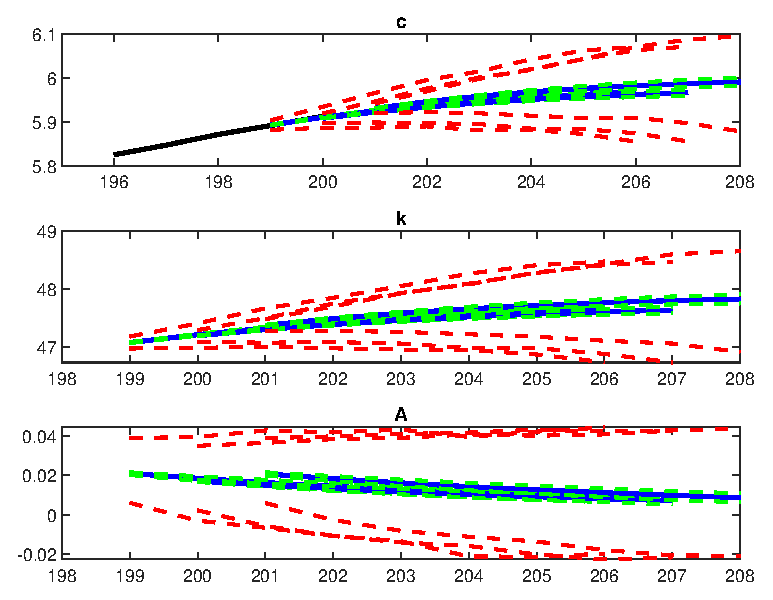
\includegraphics[width=\textwidth]{examples/rbc_basic_recursive_estimation_200/graphs/rbc_basic_recursive_estimation_RecursiveForecasts_1.eps}
  \end{figure}
\end{column}%
\hfill%
\begin{column}<1->{0.48\textwidth}
  \begin{itemize}
    \item Blue solid lines: $k$-step ahead mean forecasts 
    \item Black solid lines: actual data values for observables
    \item Green dashed lines: \texttt{mh\_conf\_sig} percent HPDI taking into account only parameter uncertainty
    \item Red dashed lines: \texttt{mh\_conf\_sig} percent HPDI with both parameter and future shock uncertainty
  \end{itemize}
  \end{column}%
\end{columns}

\end{frame}

\section[Perfect foresight controlled paths]{Perfect foresight conditional forecasts}

\begin{frame}[fragile]{Perfect foresight controlled paths}{a.k.a. conditional forecast}
  
\begin{witemize}
  \item Occasionally, scenario analysis is less interested in quantifying uncertainty and more in preserving full nonlinearities
  \item Dynare 7 offers a new syntax for conditional forecasts in a perfect foresight context (supersedes deprecated \texttt{det\_cond\_forecast} command)
  \item \texttt{perfect\_foresight\_controlled\_paths} block allows to flexibly define 
  \begin{enumerate}
    \item endogenous variables to be treated as exogenous 
    \item exogenous variables to be treated as endogenous
  \end{enumerate}
  in a particular period
  \item Restriction: in each period, there need to be as many endogenized as exogenized variables (as many instruments as targets)\\
  $\rightarrow$ cannot (yet) have future shocks driving earlier controlled variable
\end{witemize}

\end{frame}


\begin{frame}[fragile]{Controlled paths: Dynare code I}{\texttt{rbc\_basic\_pf\_controlled\_paths.mod.mod}}
\begin{minted}{c++}
var c k A;
varexo epsilon;
...
perfect_foresight_controlled_paths;
  exogenize k;
  periods 2;
  values 50;
  endogenize epsilon;

  exogenize k;
  periods 10;
  values 55;
  endogenize epsilon;
end;
\end{minted}
\end{frame}

\begin{frame}[fragile]{Controlled paths: features and compatibility}
  \begin{witemize}
  \item Can be combined with regular \texttt{shocks} or \texttt{mshocks} blocks
  \item Compatible with regular \texttt{perfect\_foresight\_solver} and \\
  \texttt{perfect\_foresight\_with\_expectation\_errors\_solver}
  \item Not compatible with \texttt{block} decomposition and \texttt{bytecode} representation
  \end{witemize}
\end{frame}

\begin{frame}[fragile]{Controlled paths: Dynare output}{\texttt{rbc\_basic\_pf\_controlled\_paths.mod}}
\begin{figure}
    \centering
    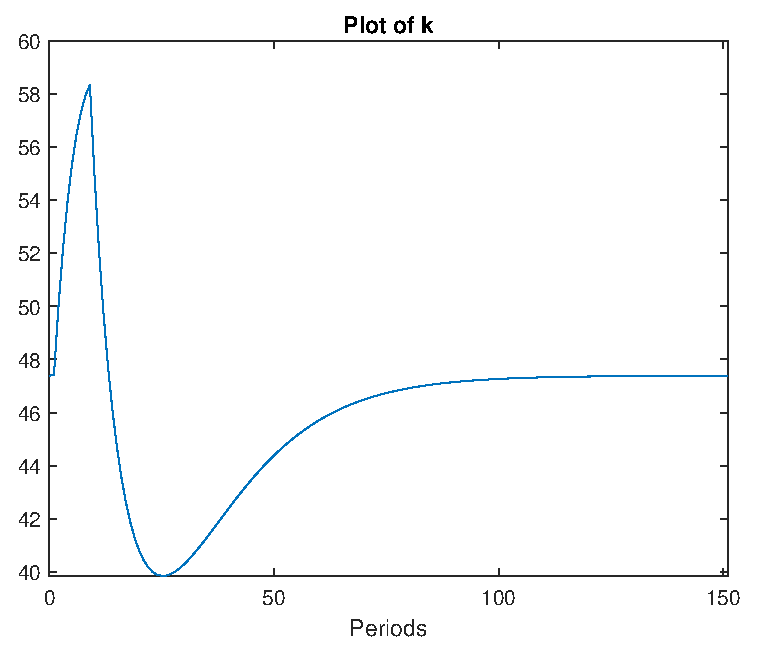
\includegraphics[width=0.35\textwidth]{examples/rbc_basic_pf_controlled_paths/graphs/SimulatedTrajectory_k.eps}
    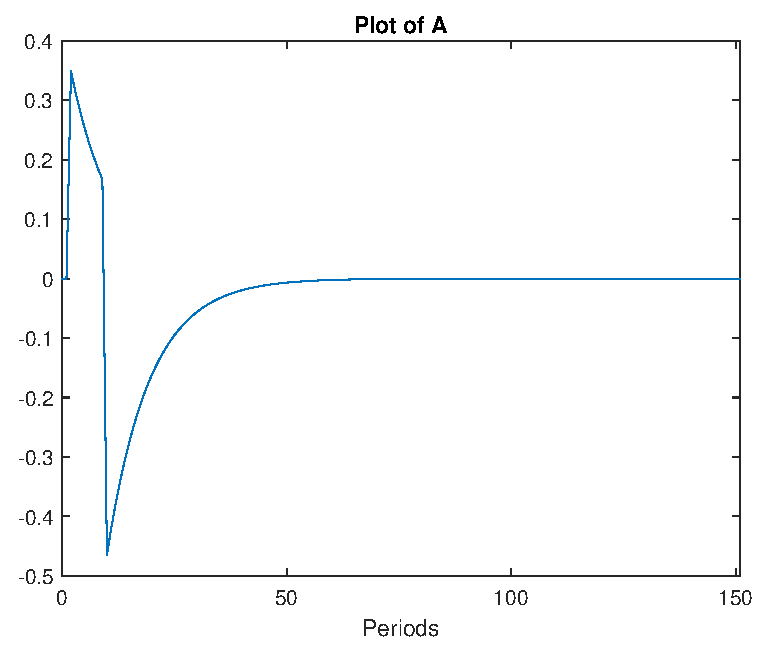
\includegraphics[width=0.35\textwidth]{examples/rbc_basic_pf_controlled_paths/graphs/SimulatedTrajectory_A.eps}
  \end{figure}
\begin{minted}{c++}
perfect_foresight_setup(periods=200);
perfect_foresight_solver;
rplot k;
rplot A;
\end{minted}
\end{frame}


\begin{frame}[plain,allowframebreaks]{References}
  \printbibliography
\end{frame}

\end{document}
